% \begin{itemize}
%     \item \textit{Chatbot};
%     \item \textit{Askubuntu};
%     \item \textit{Webapps}.
% \end{itemize}


% \begin{itemize}
%     \item mBERT;
%     \item XLM-RoBERTa.
% \end{itemize}

% \begin{itemize}
%     \item oriģinālvalodā;
%     \item mašīntulkojumā uz angļu valodu.
% \end{itemize}


% \begin{itemize}
%     \item uz tās pašas valodas korpusa;
%     \item uz visu piecu valodu korpusa;
%     \item tikai uz angļu valodas korpusa.
% \end{itemize}


Vislabākie nodomu noteikšanas precizitātes rezultāti ir \textit{Chatbot} datu kopā, tālāk iet \textit{Askubuntu} un \textit{Webapps}. Tādā pašā secībā iet šīs datu kopas pēc korpusa apjoma (206, 162 un 89 lietotāju ievadi attiecīgi), un līdzīgi sadalās piemēru skaits vienam nodomam. \textit{Chatbot} datu kopā visu metožu (izņemot 3b) vidējie rezultāti ir būtiski pārāki par \textit{Askubuntu} un \textit{Webapps} rezultātiem. Vairāk datu ir lielāka ietekme (\textit{impact}) uz precizitāti nekā vislabākās metodes izvēle.

mBERT jēdzientelpām ir labāka precizitāte \textit{Askubuntu} un \textit{Webapps} datu kopās, bet XLM-RoBERTa ir labāka precizitāte \textit{Chatbot} datu kopā.

Mašīntulkošana uz angļu valodu ir izdevīga stratēģija (četri a metožu labākie vidējie rezultāti pret diviem b, skat. \ref{tab:avg-method}. tabula). Lai arī nodomu noteikšanas korpusā visas valodas ir vienādi pārstāvētas, daudzvalodu jēdzientelpu modeļi ir apmācīti uz procentuāli lielākas daļas angļu valodas teksta. Mašīntulkošanas pārākums par oriģinālvalodu šajā kontekstā ir interesants, jo mašīntulkošana rada papildu trokšņus un kļūdas un ``pazaudē tulkojumā" katrai valodai svarīgās nianses, kas var ietekmēt ievades datu kvalitāti.

Skaitliski mazākās datu kopās (\textit{Askubuntu} un \textit{Webapps}) apvienot treniņdatus vienā korpusā ir laba ideja, trijos no četriem gadījumiem labākais vidējais rezultāts bija metodē, kurā ne-angļu treniņdati tika mašīntulkoti uz angļu valodu.  

3a metodei, neskatoties uz salīdzinošu zemu precizitāti, ir svarīga priekšrocība: tā ir vislētāk implementējama praksē, jo tai nav nepieciešami apmācības dati daudzās valodās un pietiek tikai ar angļu valodas datiem. Stabili vissliktākā metode ir 3b: apmācīt datus tikai uz angļu valodas korpusa un testēt uz korpusa citā valodā, pirms tam netulkojot uz angļu valodu. Iespējams tas ir saistīts ar šo korpusu specifiku (maz datu). Taču 3b ir interesanta metode, jo parāda starpvalodu mācīšanos.

Līdzīgu datu korpusu gadījumā virtuālajam asistentam autore izvēlētos trenēt vienu nodomu klasifikācijas modeli, kas apmācīts uz datiem, kas ir mašīntulkoti uz angļu valodu un apvienoti vienā korpusā.


Salīdzinot darbā iegūto nodomu noteikšanas precizitāti angļu valodā ar literatūrā pieejamo \cite{fasttext2019}, var secināt, ka darbā izmantotie modeļi pārspēj dažus no komerciāli piedāvātajiem variantiem (\ref{fig:comparison} attēls). Tomēr jāņem vērā, ka literatūras datos, atšķirība no šī darba, nodomi ar mazāku piemēru skaitu netika apvienoti "\textit{Other}" nodomā.

% Datu kopas



% Table generated by Excel2LaTeX from sheet 'Sheet1'
% \begin{table}[htbp]
%   \centering
%   \caption{Add caption}
%     \begin{tabular}{rlrrrrrr}
%           &       & \multicolumn{1}{l}{1a} & \multicolumn{1}{l}{1b} & \multicolumn{1}{l}{2a} & \multicolumn{1}{l}{2b} & \multicolumn{1}{l}{3a} & \multicolumn{1}{l}{3b} \\
%     \multicolumn{1}{l}{chatbot} & mbert & 91.39 & 92.03 & 92.16 & 92.08 & \textbf{92.57} & 81.98 \\
%           & roberta & 90.45 & 91.93 & 92.69 & \textbf{93.54} & 91.16 & 84.62 \\
%     \multicolumn{1}{l}{askubuntu} & mbert & 79.87 & \textbf{81.10} & 79.24 & 79.95 & 79.36 & 62.84 \\
%           & roberta & 66.92 & 68.90 & \textbf{77.12} & 76.74 & 68.75 & 52.94 \\
%     \multicolumn{1}{l}{webapps} & mbert & 64.72 & 63.14 & \textbf{73.20} & 67.29 & 62.71 & 42.71 \\
%           & roberta & 43.64 & 49.24 & \textbf{66.31} & 66.10 & 48.62 & 35.85 \\
%     \end{tabular}%
%   \label{tab:addlabel}%
% \end{table}%



\begin{table}[htbp]
  \centering
  \caption{Visu valodu vidējie rezultāti katrai metodei visās jēdzientelpās un datu kopās, \%.}
    \begin{tabular}{rlrrrrrr}\toprule
          &       & 1a    & 1b    & 2a    & 2b    & 3a    & 3b \\\midrule
    \textit{Chatbot} & mBERT & 91.39 & 92.03 & 92.16 & 92.08 & \textbf{92.57} & 81.98 \\
          & XLM-RoBERTa & 90.45 & 91.93 & 92.69 & \textbf{93.54} & 91.16 & 84.62 \\\midrule
    \textit{Askubuntu} & mBERT & 79.87 & \textbf{81.10} & 79.24 & 79.95 & 79.36 & 62.84 \\
          & XLM-RoBERTa & 66.92 & 68.90 & \textbf{77.12} & 76.74 & 68.75 & 52.94 \\\midrule
    \textit{Webapps} & mBERT & 64.72 & 63.14 & \textbf{73.20} & 67.29 & 62.71 & 42.71 \\
          & XLM-RoBERTa & 43.64 & 49.24 & \textbf{66.31} & 66.10 & 48.62 & 35.85 \\\bottomrule
    \end{tabular}%
  \label{tab:avg-method}%
\end{table}%


\begin{figure}[h]
   \centering
   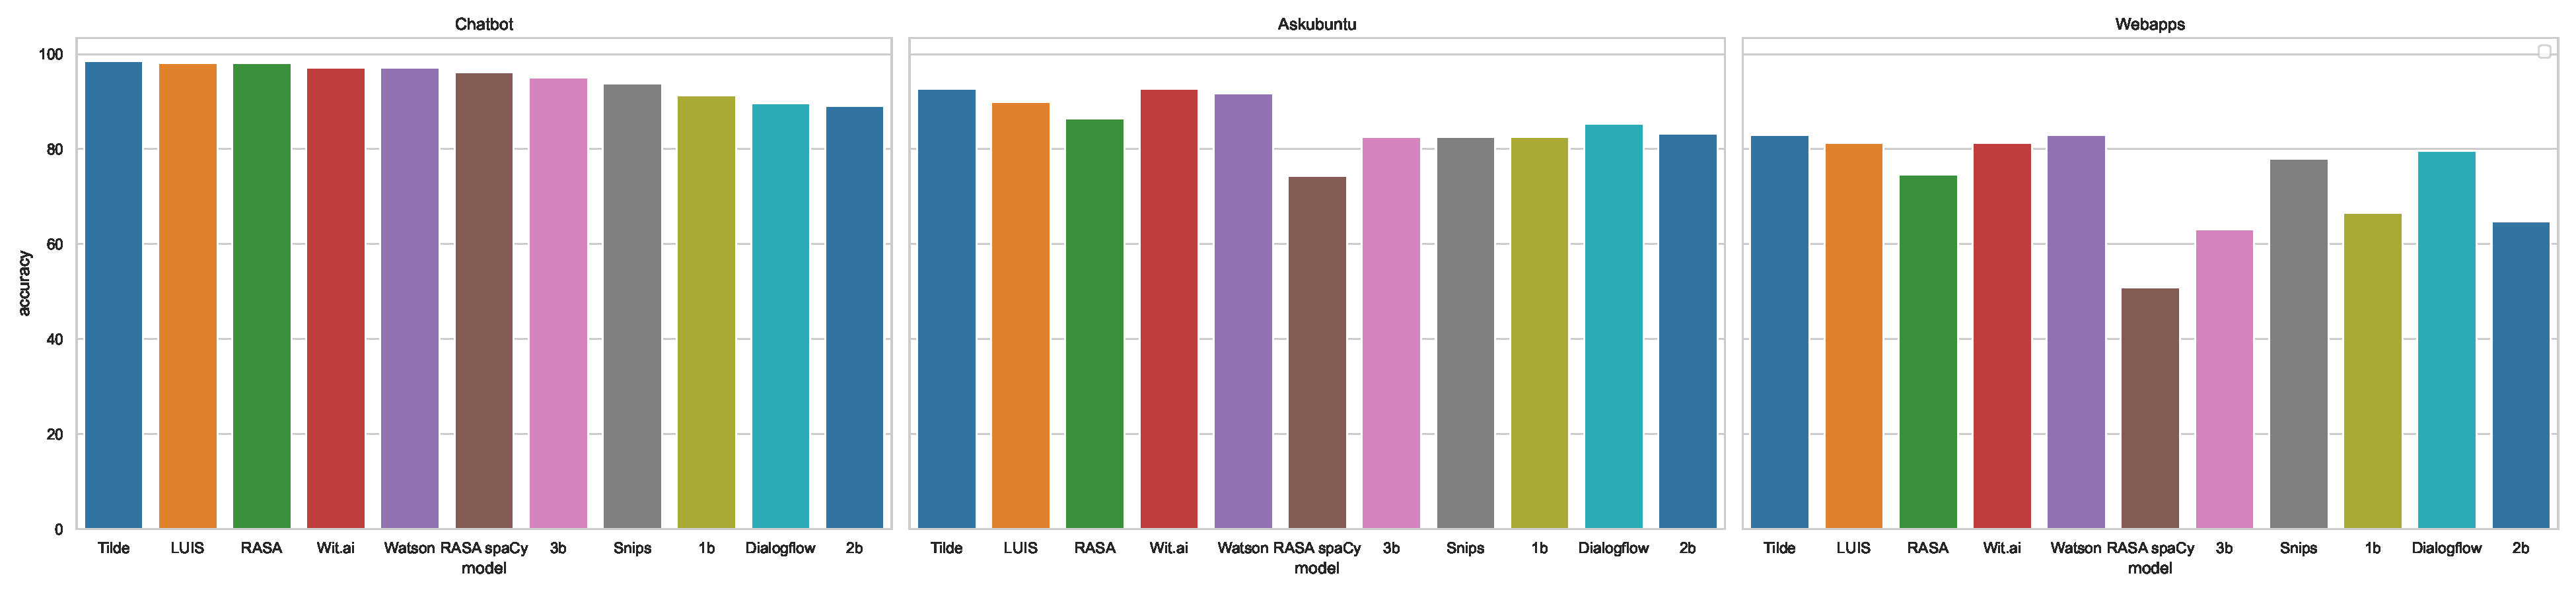
\includegraphics[width=\linewidth]{figures/results.pdf}
   \caption{Vairāku dialogu sistēmu nodomu noteikšanas precizitāte angļu valodā, \%, (dati \cite{fasttext2019}).}
   \label{fig:comparison}
\end{figure}